In order to test the equations and design outlined in the Theory section above, the mathematics was implemented in a script written in the Python programming language and developed in the PyCharm IDE. The program consists of a GUI  used to enter elementary commands, similar to that implemented in the Android application, as well as a window for plotting the result in a 3-dimensional Cartesian system. Some results showing the validity of the design equations in the previous section can be found below. All of the source code used to build this simulation can be found in Part 5 of this report on the attached optical disc.\\

The program flow of the software in the simulation is similar to that used for the final prototype software, more information on the software design flow can be found in Section \ref{sec:soft}. The main difference between the final implementation and the simulation is that once the angle values for theta, alpha and phi are calculated for each leg, in the final implementation the result is used to move the actuator while in simulation the result is used to calculate the Cartesian position of each limb in order to plot it in the 3-dimensional system. It should be noted that the length of all of the limbs as well as the robot body radius was chosen as unity for simplicity and since the purpose of the simulation is only to show the functionality of the IK. It should also be noted that although some of the legs may look crooked in the following figures, this is only a result of the viewing angle. When viewed directly from above, all limbs of a single leg align in an upright plane.\\

The basic user interface together with the Robot in its neutral position can be seen in Figure \ref{fig:Sim1}.\\

The orange markers found at each of the robot feet indicate the neutral position for each of the five feet. This is indicated to aid in showing the movement of the legs relative to this neutral position in Figure \ref{fig:Sim1} and the figures following in this section.\\

\begin{figure}[H]
\centering
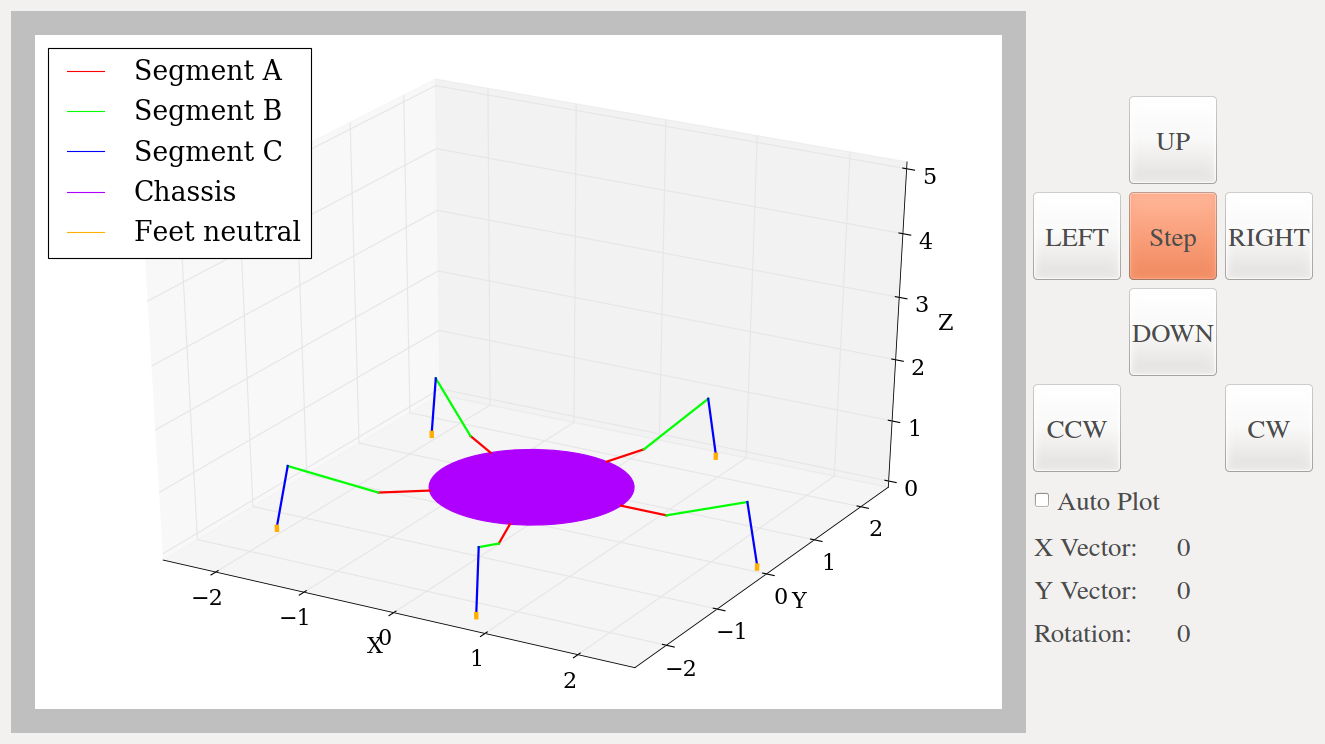
\includegraphics[scale = 0.33]{pics/Sim1.png}
\caption{Simulation window showing the robot in its neutral position.}
\label{fig:Sim1}
\end{figure}

When the $Y$ vector is changed to a positive value, the legs will all move in a negative $Y$-direction since the robot center is the origin. When the robot should move in a specific direction, the feet will move in the exact opposite direction to propel the robot forward. This is illustrated in Figure \ref{fig:Sim2}.

\begin{figure}[H]
\centering
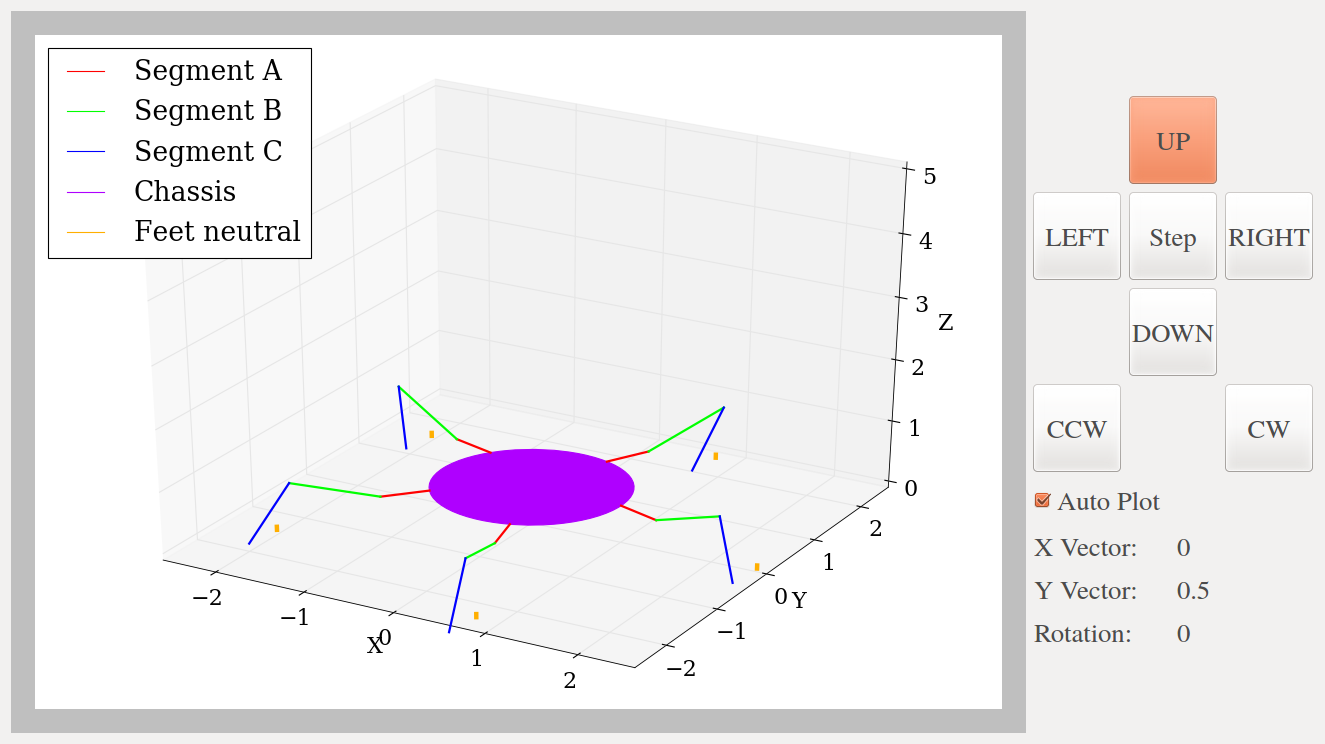
\includegraphics[scale = 0.33]{pics/Sim2.png}
\caption{Simulation window showing the robot moving in a positive $Y$-direction.}
\label{fig:Sim2}
\end{figure}

The robot should also be able to translate in the $X$-direction without making a rotation first. This is illustrated in Figure \ref{fig:Sim3}.

\begin{figure}[H]
\centering
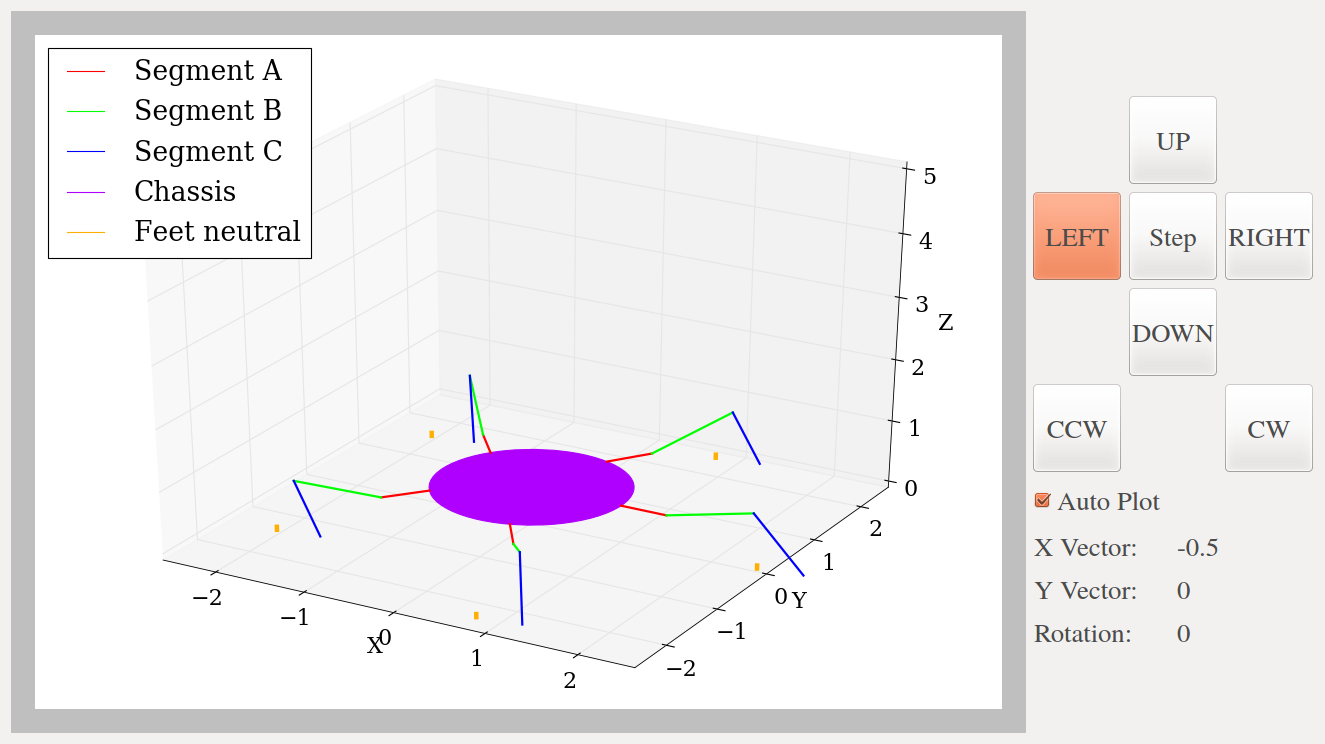
\includegraphics[scale = 0.33]{pics/Sim3.png}
\caption{Simulation window showing the robot moving in a negative $X$-direction.}
\label{fig:Sim3}
\end{figure}

If the robot can instantaneously move in both the $X$ and $Y$-directions, it should be able to move in a combination of the two without a problem. This ability is illustrated in Figure \ref{fig:Sim4}.

\begin{figure}[H]
\centering
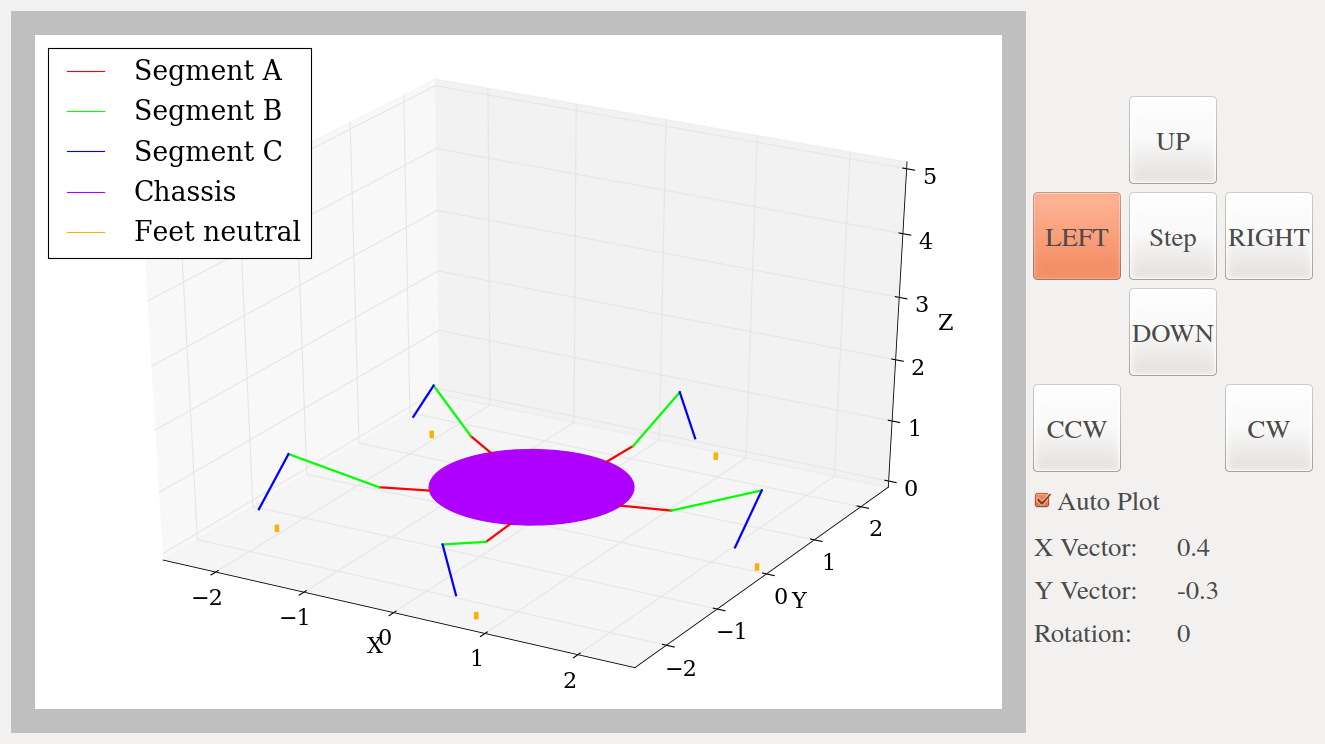
\includegraphics[scale = 0.33]{pics/Sim4.png}
\caption{Simulation window showing the robot moving in a direction with a positive $X$ and negative $Y$-component.}
\label{fig:Sim4}
\end{figure}

The translation appears to be working exactly as intended and designed for. The simulation is tested with a clockwise direction rotation in Figure \ref{fig:Sim5}.

\begin{figure}[H]
\centering
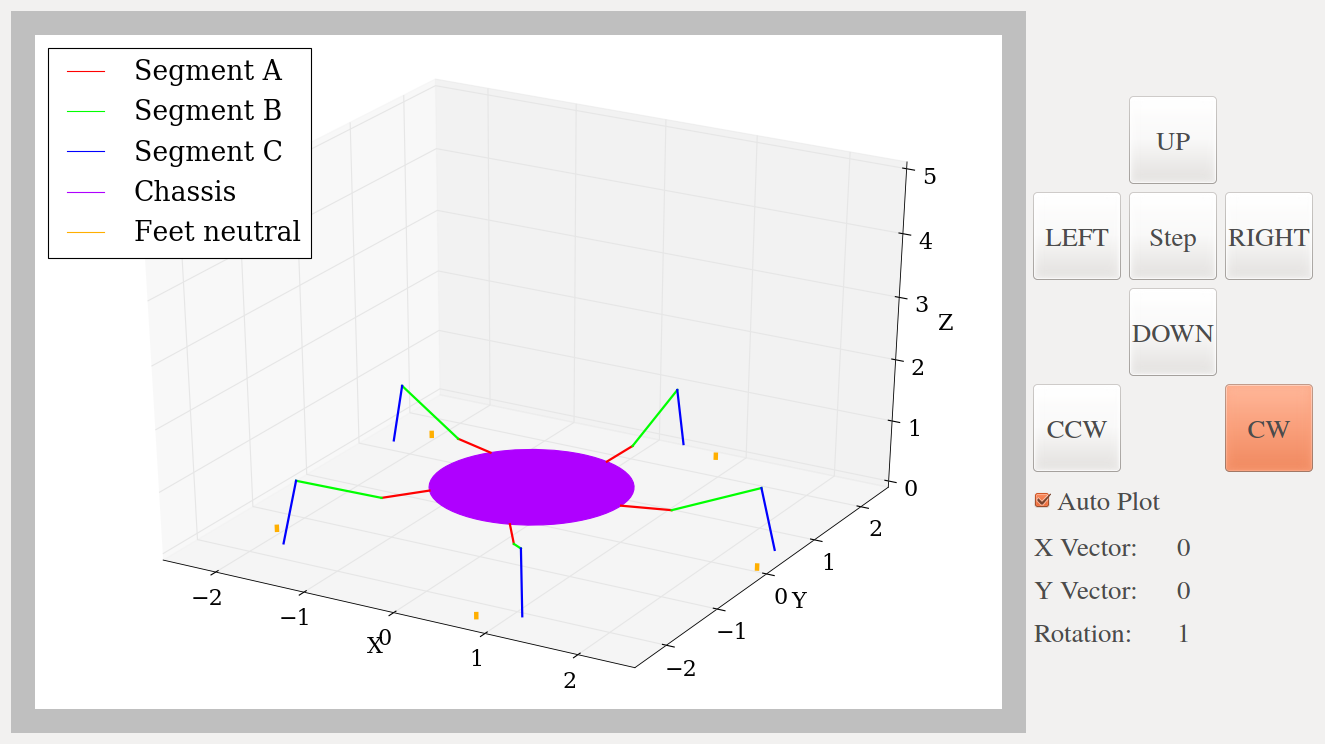
\includegraphics[scale = 0.33]{pics/Sim5.png}
\caption{Simulation window showing the robot rotating in a clockwise direction.}
\label{fig:Sim5}
\end{figure}

Once the robot reaches the boundary illustrated in Figure \ref{fig:Body_layout_3} for any of its legs, it is necessary to lift the leg up, move it to a more suitable location and put it down in order to continue in the direction it is heading in. This ability is illustrated in Figure \ref{fig:Sim6}.

\begin{figure}[H]
\centering
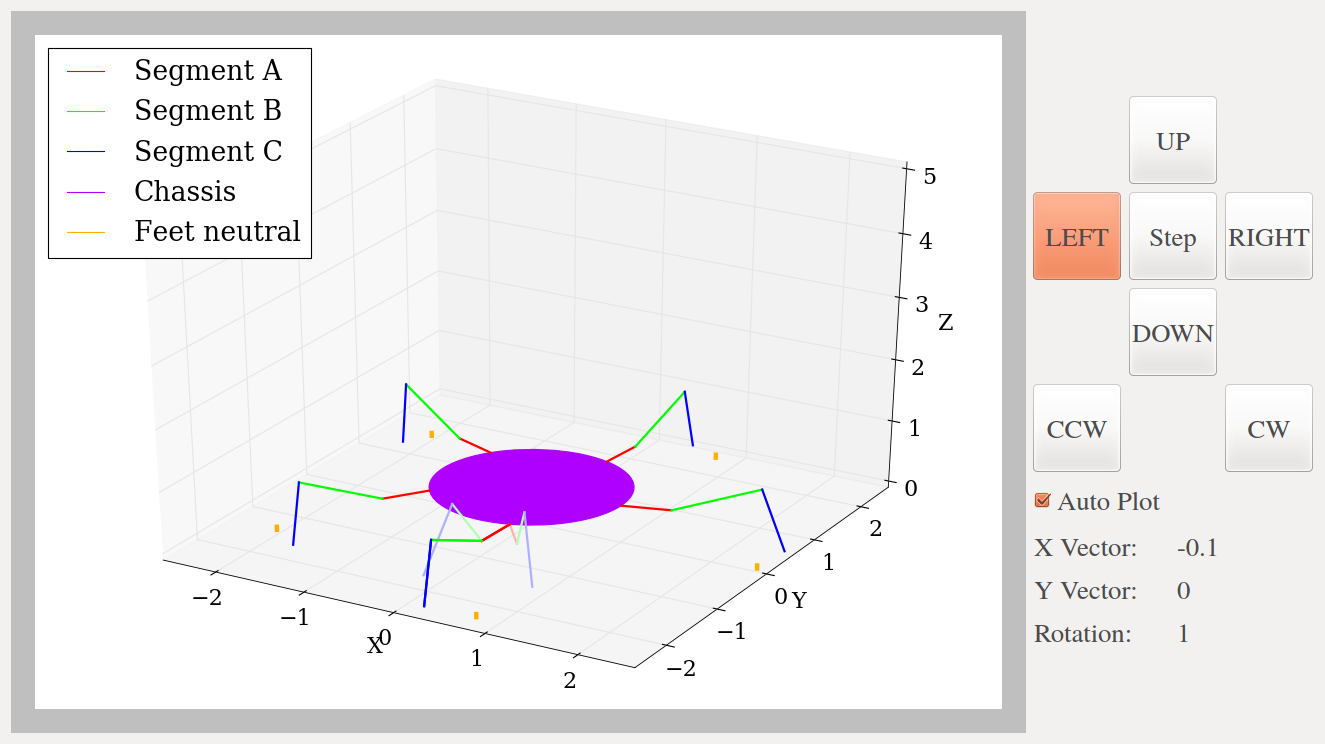
\includegraphics[scale = 0.33]{pics/Sim6.png}
\caption{Simulation window showing the robot picking up a foot and placing it again.}
\label{fig:Sim6}
\end{figure}

In Figure \ref{fig:Sim6}, the closest leg appears three times, twice in dimmed (ghost) colours and then finally in the normal colours. What this attempts to illustrate is the resetting motion of the leg. Figure \ref{fig:Sim5} shows the robot just before the resetting action. The right of the two "ghost" legs is right above the original location of the leg. This shows the position of the leg after it was lifted up. The left of the two "ghost" legs is the leg, still lifted, after being moved to a position directly over the new location. The leg plotted in full colour shows the final position of the leg. It is now able to start rotating further in the clockwise direction. Th robot will pickup and replace one leg at a time for all the legs that requires resetting and then continue.
